\documentclass[11pt]{article}
\usepackage[utf8]{inputenc}
\usepackage[french]{babel}
\usepackage[margin=3cm, paperwidth=21cm, paperheight=29.7cm]{geometry}
\usepackage{graphicx}
\usepackage{SIunits}
\usepackage{tabto}
\usepackage{eurosym}
\usepackage{subcaption}
\usepackage{hyperref}
\hypersetup{hidelinks}
\usepackage{url}
\usepackage{listings}
\usepackage[footnote]{acronym}
\usepackage[T1]{fontenc}
\usepackage{array}
\usepackage{wrapfig}
\usepackage{lipsum}
\usepackage{float}

\renewcommand{\contentsname}{Table des matières}
\begin{document}
\begin{titlepage}
    \begin{center}
    \huge{\textbf{M2 EEA SME}}\\[0.5 cm]
    {\large Projet Barre Franche - Novembre 2019}\\[0.5cm]
    
    % Title
    \rule{\linewidth}{0.5mm} \\[0.4cm]
    {\huge \bfseries EIEAS3GM \\ SYNTHESE ET MISE EN ŒUVRE DES SYSTEMES\\[0.4cm]}
    \rule{\linewidth}{0.5mm} \\[1.5cm]
    
    % Title
    
    % Author and supervisor
    
    \begin{center}
    \begin{minipage}[t]{0.46\textwidth}
      \begin{flushleft} \large
        \textbf{Auteur :}\\
        Nicolas OTAL\\
        Antoine ROUTIER\\
      \end{flushleft}
    \end{minipage}
    \begin{minipage}[t]{0.46\textwidth}
      \begin{flushright} \large
        \textbf{Encadrants :}\\
        M. PERISSE\\
      \end{flushright}
    \end{minipage}
    \end{center}
    
    \vfill
    
    %%%%%%%%%%%%%%%%%%%%%%%%%
    %%% Bottom First page %%%
    %%%%%%%%%%%%%%%%%%%%%%%%%
    
    \begin{figure}[b]
    \centering
    
\includegraphics[width=0.65\textwidth]{images/Upstls.jpg}
    \end{figure}
    
    \end{center}
    \end{titlepage}
\newpage
\setcounter{page}{2}
\section*{Introduction}
\label{Introduction}
\addcontentsline{toc}{section}{\nameref{Introduction}}
\textit{Dans le cadre de notre UE "Synthèse et Mise en oeuvre de système", un bureau d'étude nous a été proposé avec pour objectif de mettre en oeuvre une solution logicielle/matérielle qui répond au besoin de gestion et contrôle de trajectoire d'un voilier de barre franche.}\\

\textit{A l'aide des bases acquises, durant notre formation, en VHDL, simulation, et conception systèmes l'objectif de cette UE sera la réalisation d'un contrôleur de Barre-France de voilier par FPGA (Altera). Il sera nécessaire d'étudier, décomposer, coder et implémenter chaque fonctions une à une et d'intégrer la globalité du projet à l'aide d'un Bus Avalon permettant l'interconnexion des fonctions au MCU intégré au FPGA.}\\

\textit{Pour réaliser cela, nous avons respecter le processus de développement consistant à réaliser une analyse  des besoins et du contexte permettant d'identifier les différentes interfaces du système, nous avons par la suite réaliser la conception du système en décomposant notre fonction principale en différents blocs. Ces différents blocs ont fait l'objet d'une description fonctionnelle avant d'être implémenter. Suite à cela, nous avons réaliser un ensemble de simulation et test sur maquette pour vérifier le bon fonctionnement de chaque module intégré pour valider finalement notre projet sur une maquette.}
\newpage
\renewcommand{\thepage}{\arabic{page}}

\textbf{\LARGE{Sigles et acronymes}}\\
\begin{acronym}[CP-OFDMX] % Give the longest acronym here
\acro{FPGA}{\emph{Field Programmable Gate Arrays}} 
\acro{GPIO}{\emph{General Purpose Input/Output}} 
\acro{GPS}{\emph{Global Positioning System}} 
\acro{NMEA}{\emph{National Marine Electronics Association}} 
\acro{SOPC}{\emph{System On Programmable Chip}} 
\acro{SRAM}{\emph{Static Random Access Memory}} 
\acro{UART}{\emph{Universal Asynchronous Receiver Transmitter}}
\acro{VHDL}{\emph{VHSIC Hardware Description Language}}
\acro{VHSIC}{\emph{Very High Speed Integrated Circuits}}
\end{acronym}
\newpage

\tableofcontents
\newpage

\section{Cahier des charges du Projet "Barre-Franche"}
\subsection{Introduction technique}
Le projet qui nous est demandé est basé sur les SOC et plus particulièrement sur un FPGA, de chez Altera, embarqué dans un voilier pour en piloter la barre-franche.
\newline
Ce dispositif électronique fonctionnera à l'aide de différentes entrées/sorties (gyroscope, anémométre, GPS, convertisseur analogique/numérique, vérin, boutons, buzzer).
\subsection{Cahier des charges général}
Durant ce projet, nous allons utiliser les différentes compétences acquises à travers les différents cours de l'année et les mettre en corélation pour mener à bien ce dernier. Le projet devra respecter certains critères présentés ci-dessous :
\begin{enumerate}
    \item   Le dispositif devra utiliser un appareil de mesure pour capter la valeur de la vitesse du vent.
    \item   Le dispositif devra utiliser un appareil de mesure pour capter la direction du vent.
    \item   Le dispositif devra receptionner des données GPS, traiter ces données et agir sur le dispositif en fonction des résultats obtenus après traitement.
    \item
\end{enumerate}
\subsection{Cahier des charges technique}




\section{Conception Matérielle}
Pour mettre en oeuvre les différentes parties du projet combinatoires et séquentielles, nous avons du passer par des étapes d'analyses comportementales de chaque blocs à réaliser pour ainsi créer des composants simples pouvant être utilisés à la composition de fonctions plus complexes plus tard. L'implémentation de chaque composants a été réalisée grâce au langage VHDL sur le logiciel de développement Quartus.

Ainsi nous avons réalisé différentes "boîtes" de composants simples pour réaliser des fonctions entières, et plus complexes, contenant les blocs simples.

\subsection{Réalisation fonction simple - Gestion anémomètre}
La fonction réalisant l'acquisition de la vitesse du vent (0 à 250 Km/h) se fait à l'aide d'un anémomètre qui sert de transducteur convertissant la vitesse du vent en fréquence variable (0 à 250 Hz). 
\vspace{0.5cm}\\
Le composant doit fonctionner selon deux modes :
\begin{enumerate}
    \item Mode continu, dans ce mode le système actualise l'acquisition toutes les secondes de la vitesse du vent. Pour cela, l'entrée "Continu" doit être à 1. 
    \item Mode mono-coup, dans ce mode le système effectue qu'une seule acquisition lorsque "Start/Stop" est activé. Une fois "data\_valide" envoyé le système remet les entrées "Start/Stop" et "data\_valide" à zéro après une acquisition et attend la prochaine entrée "Start/Stop".
\end{enumerate}
\vspace{0.5cm}
La figure 3 représente la décomposition des composants utilisés pour la réalisation du bloc "Captage force vent". 

\begin{figure}[h]
    \begin{center}
      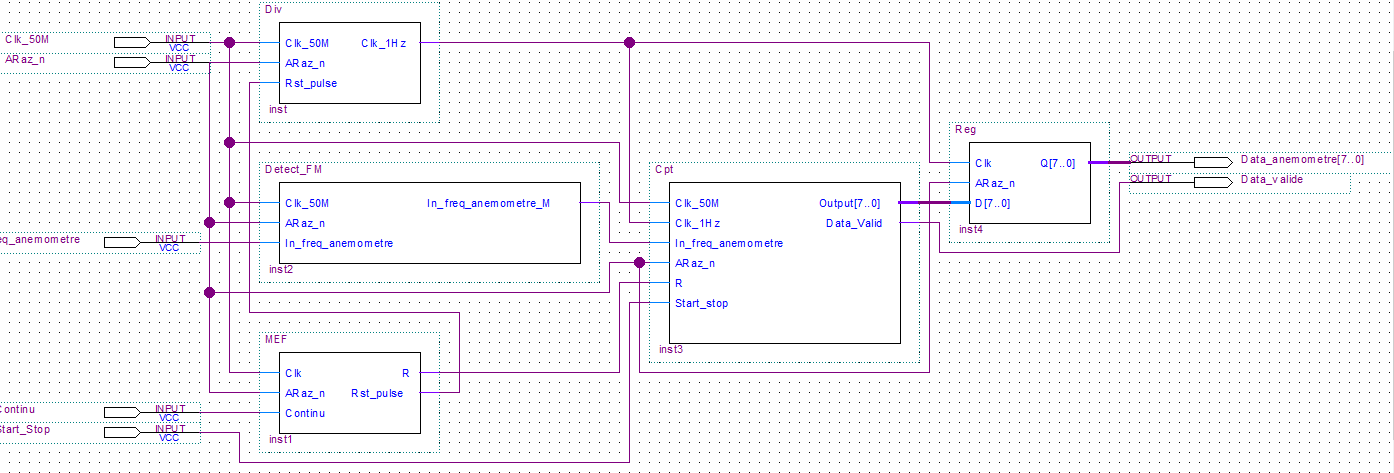
\includegraphics[width=\textwidth]{images/captation.png}
      \caption{Diagramme fonctionnel du circuit "Captation vitesse vent"}
    \end{center}
  \end{figure}

  Le composant "Div" fournit une horloge de 1 Hz à partir de l'horloge 50 MHz donnée par la clock du FPGA. L'horloge de 1 Hz sera utilisée pour l'acquisition de la fréquence de l'anémomètre toutes les secondes.

\newpage

  Le deuxième composant "Detect\_FM" est en charge de détecter les fronts montants sortant de l'anémomètre pour transformer la fréquence générée en Hertz en une donnée interprétable par le composant "Cpt".\\\newline

  Le composant "Cpt" va permettre de récupérer la quantité de fronts montants comptés par le composant "Detect\_FM", toutes les secondes quand le composant sera en mode continue et une seule fois lors du mode mono-coup.\\\newline

  Le composant "Reg" permettant de stocker la valeur de la fréquence convertie dans un registre ce qui va permettre de venir traiter ou effectuer des calculs une fois celle-ci acquise (ici dans le MCU qui sera réalisé prochainement).\\\newline

  Le composant "MEF" est chargé de gérer le mode de fonctionnement du circuit, ce qui permet à ce bloc fonctionnel de savoir quand il doit être remis à zéro ou savoir quand il est en mode "Continu" ou "Mono-coup".\vspace{1cm}
  \begin{figure}[h]
    \begin{center}
      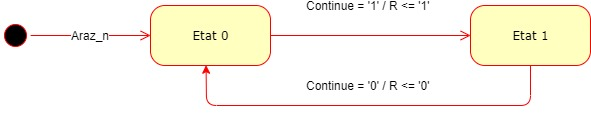
\includegraphics[width=\textwidth]{images/MEF_anemo.jpg}
      \caption{Machine à états Gestion anémomètre}
    \end{center}
  \end{figure}

Au projet, une partie interface Avalon a été ajoutée permettant l'implémentation et l'interfaçage des fonctions entre la partie NIOS II et la partie matérielle FPGA. 
  \newpage

  \subsection{Réalisation fonction complexe - Gestion vérin}

  La fonction réalisant le mouvement de la barre franche est réalisé avec le circuit vérin. Ce circuit est composé de 3 fonctions principales qui vont permettre le pilotage du vérin qui contrôle la barre franche du voilier :\vspace{0.5cm}
\begin{enumerate}
    \item Une gestion d'un signal PWM effectué par le process "PWM" qui va permettre de faire sortir ou rentrer le vérin en fonction d'une fréquence et le rapport cyclique. 
    \item Un contrôle des butées réalisé par le process "Gestion\_Butée" qui sous certaines conditions fixées dans la partie logicielle du projet fera l'avance ou le recul du vérin jusqu'à celles-ci.
    \item Une machine à états pour la gestion du convertisseur MCP3201 12 bits rendant possible le déplacement du vérin dans un sens puis dans un autre.
    \item Une partie interface Avalon est ajouté au projet pour créer le lien entre la partie logicielle et la partie matérielle du FPGA/NIOS II.
\end{enumerate} 

  \begin{figure}[h]
    \begin{center}
      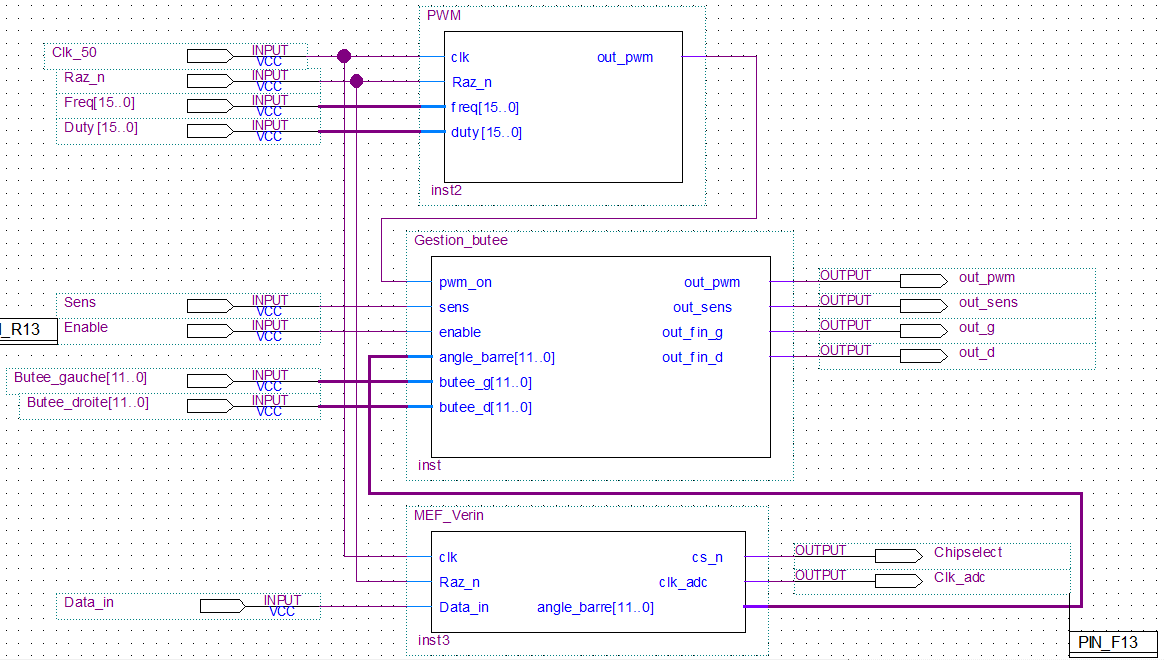
\includegraphics[width=\textwidth]{images/verin.png}
      \caption{Diagramme fonctionnel du circuit "Actionnement Barre"}
    \end{center}
  \end{figure}

\newpage 

La machine à états ci-dessous décrit le comportement du bloc Gestion vérin permettant ainsi de gérer le pilotage du convertisseur AN MCP3201 qui va mémoriser la donnée "angle\_barre" pour ensuite l'écrire sur le bus du NIOS II puis dans des régistres.
\vspace{1cm}
  \begin{figure}[h]
    \begin{center}
      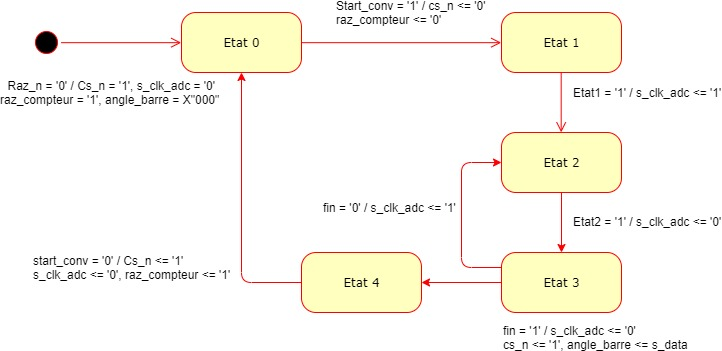
\includegraphics[width=\textwidth]{images/MEF_verin.jpg}
      \caption{Machine à états Gestion vérin}
    \end{center}
  \end{figure}

  \newpage

  \subsection{Réalisation Asservissement vérin (Compas + Interface)}	
Après l'implémentation des fonctions simple et complexe le temps nous a permit d'instancier l'asservissement du vérin en y ajoutant l'interface Homme système (boutons, Leds et buzzer) ainsi que la partie compas nécessaires à l'asservissement. Nous avons par manque de temps copié les fonctions déjà présente sur le site du projet mais avons développé nous mêmes les parties centrales pour éviter de copier un projet sans le comprendre. Les machines à états développées dans les fichiers VHDL sont donc développées par nous mêmes. 	

\vspace{1cm}	
  \begin{figure}[h]	
    \begin{center}	
      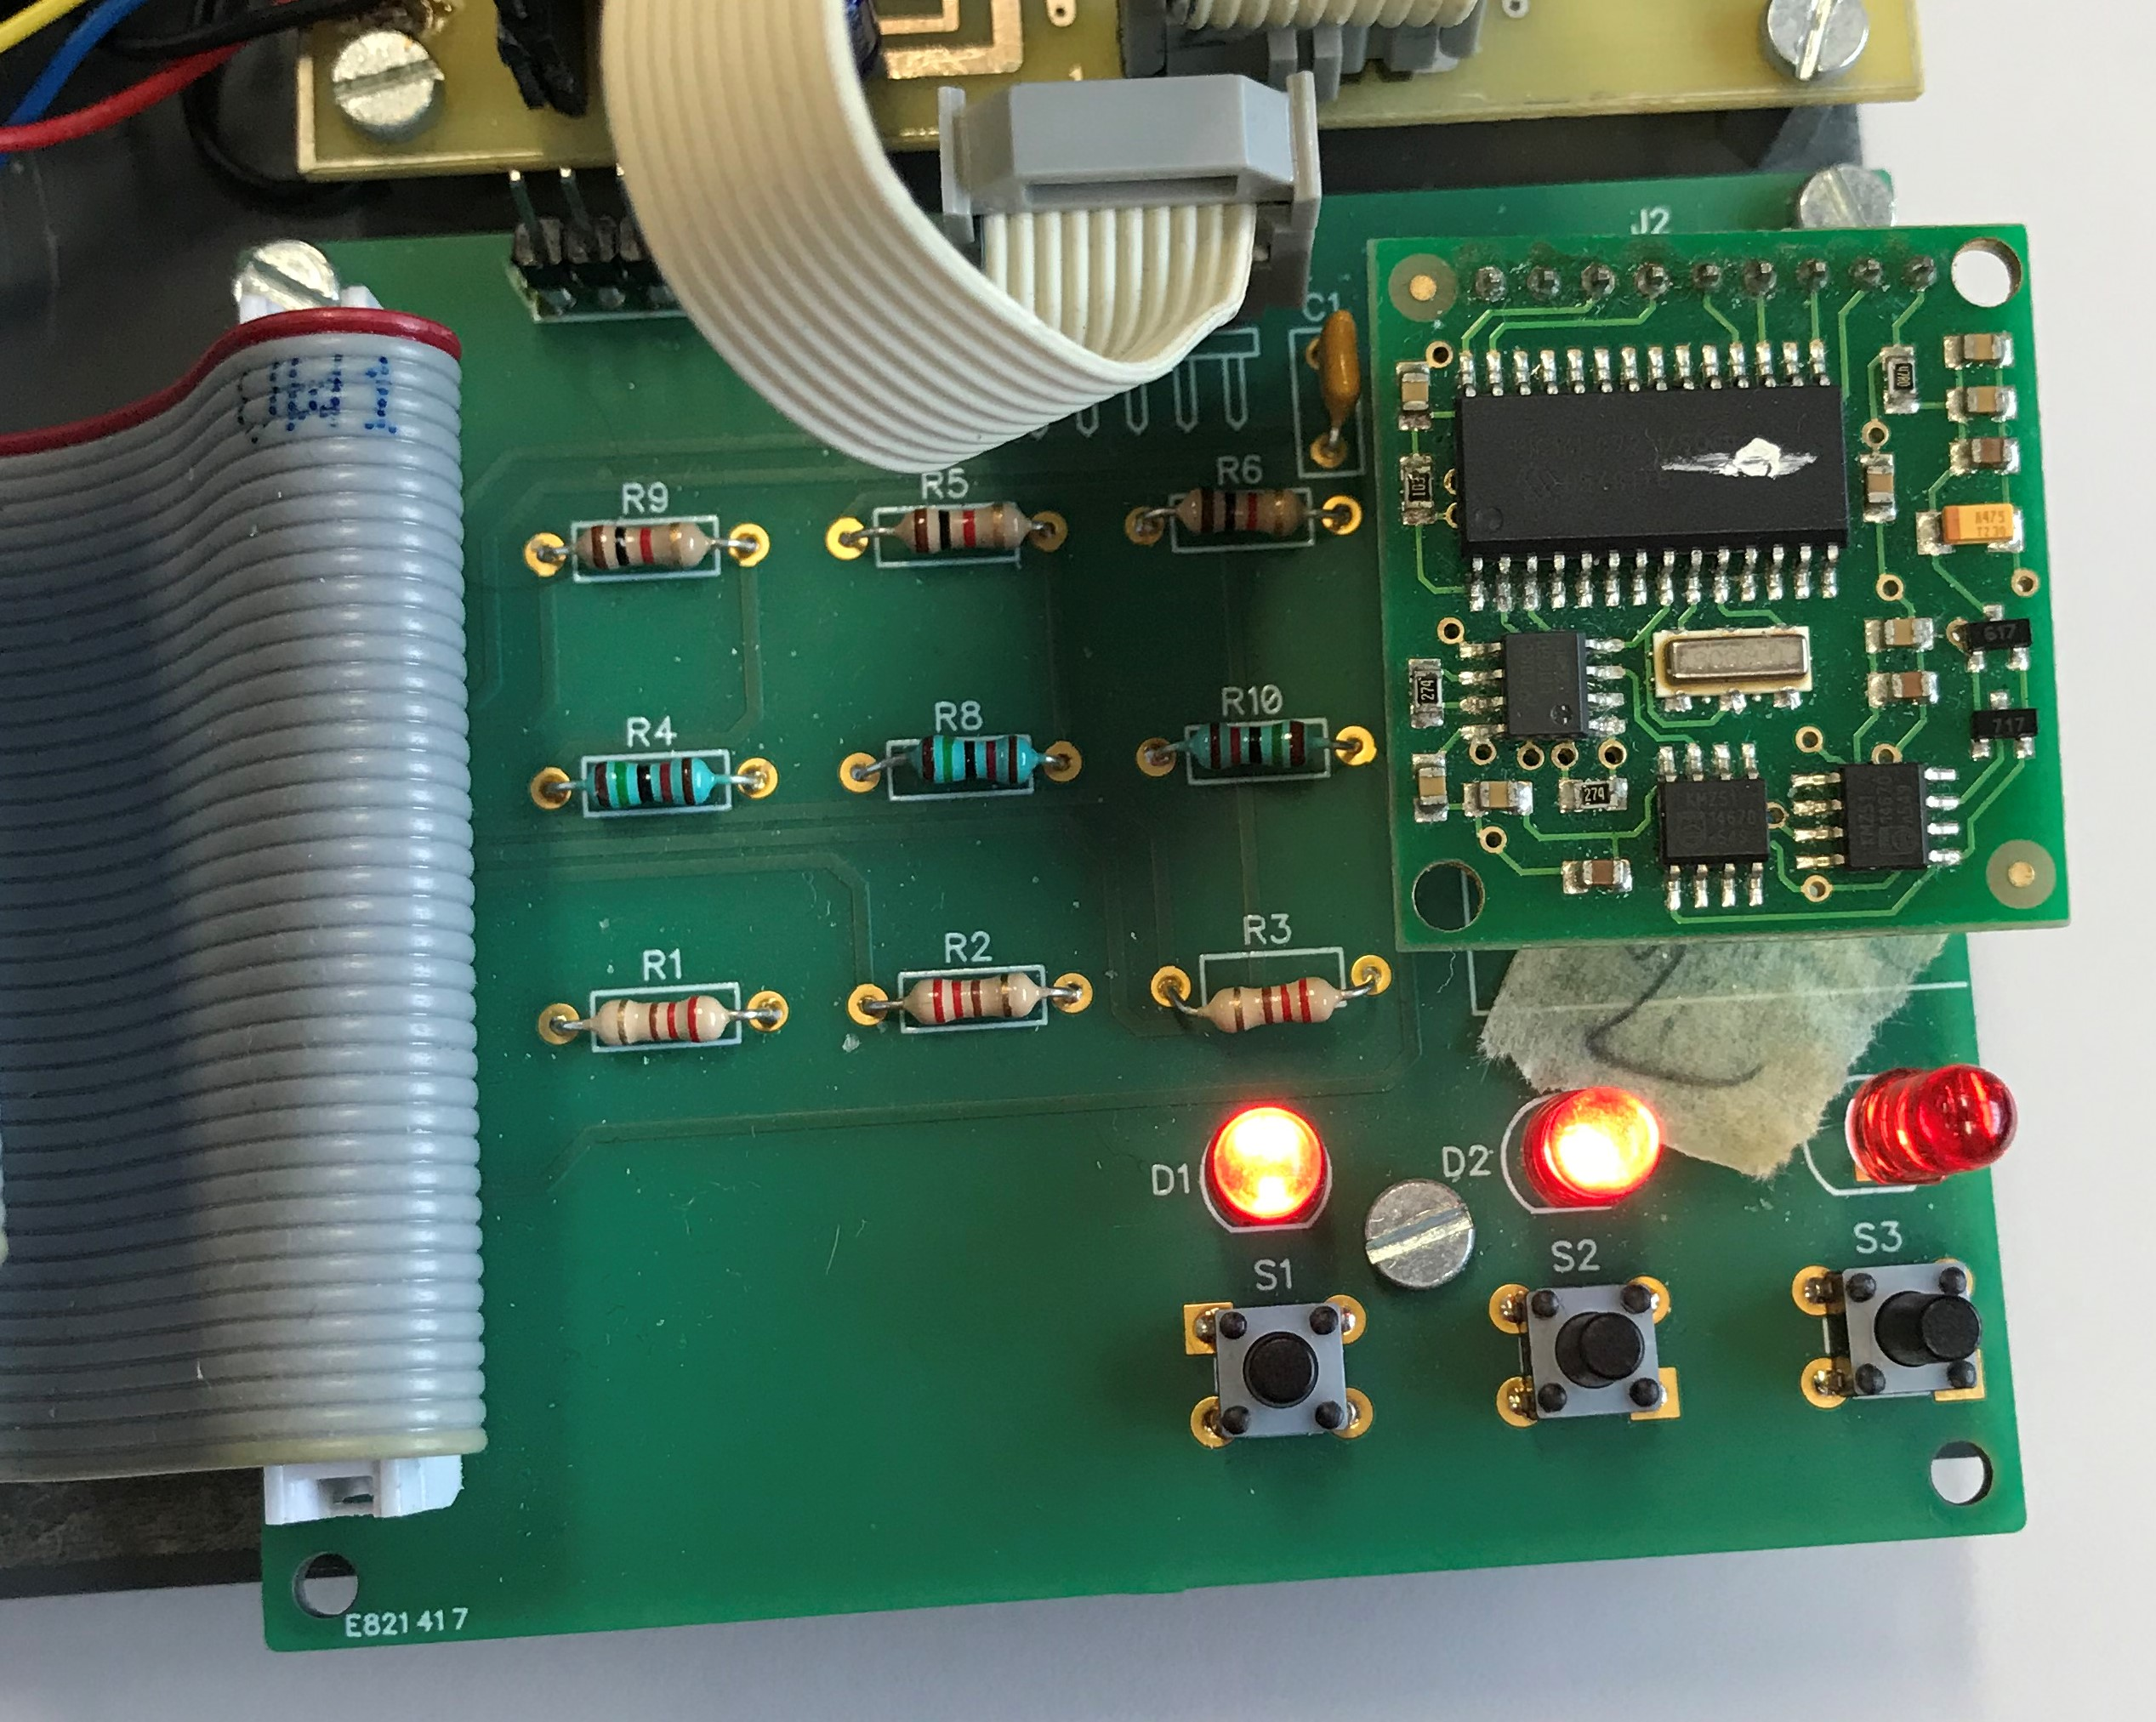
\includegraphics[width=0.5\textwidth]{images/bp.jpg}	
      \caption{Boutons poussoir, leds et buzzer}	
    \end{center}	
  \end{figure}	

  La partie compas développée nous a permit d'intégrer le composant CMPS03 qui est une boussole I2C (module à droite de la figure 7). Ce module va nous permettre dans l'asservissement de définir un cap à suivre pour le voilier. Ce bloc fonctionnel est complémenté par le bloc interface qui va permettre durant l'asservissement de corriger (+1/+10 degrés ou -1/-10 degrés) et d'afficher le cap que suit le voilier. Le passage du mode manuel vers le mode automatique se fera aussi à l'aide de l'interface implémentée en fin du bureau d'étude (en bas de la figure 7). 	

  \newpage

  \subsection{Réalisation interfaces Avalon}

La création d'une interface processeur et matériel programmable est nécessaire au bon fonctionnement du projet. Altera a développé un bus informatique appelé bus "Avalon" destiné à l'implémentation matériel/composants sur FPGA. Il va permettre l'interconnexion entre le processeur NIOS II (réalisé à l'aide de SOPC builder) et les périphériques des différents composants que nous avons créé ultérieurement.\\
\newline
Pour réaliser cette interface il a fallut respecter le cahier des charges donné en début de projet pour chaque interfaces, qui correspondent à des circuits combinatoires/séquentiels utilisés pour l'écriture et la lecture du bus (Address, read, write, chip select...). Ci-dessous sont représentés les différents circuits que nous avons implémenté au projet.\\
\newline
La première interface correspond à la fonction Anémomètre.
\begin{figure}[h]
  \begin{center}
    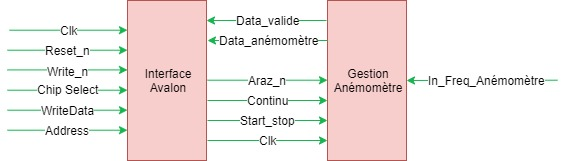
\includegraphics[width=0.8\textwidth]{images/avalon_anemo.jpg}
    \caption{Interface Avalon Gestion anémomètre}
  \end{center}
\end{figure}\\
\newline
La deuxième interface correspond à la fonction Gestion vérin.

\begin{figure}[h]
  \begin{center}
    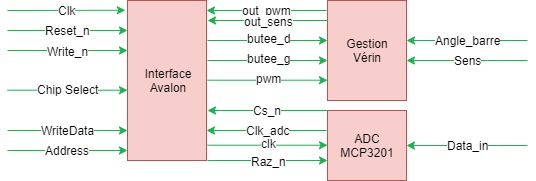
\includegraphics[width=0.8\textwidth]{images/avalon_verin.jpg}
    \caption{Interface Avalon Gestion vérin}
  \end{center}
\end{figure}

\section{Conception conjointe Matérielle/Logicielle}
La conception conjointe , est aussi appelée "codesign" qui correspond à une fonctionnalité complexe qui allie une partie logique programmée (flexibilité) et une logique câblée (performances). Utilisée pour réaliser des système complexes sur Silicium ou SOPC, dans notre cas (System On Programmable Chip) sur FPGA. Ce qui permet d'intégrer les périphérique ainsi que le processeur dans le FPGA, dans notre projet il s'agît de la réalisation d'un micrô-contrôleur.\newline

Dans le système réalisé pour le projet nous avons généré, à l'aide de "SOPC Builder", un système SOPC comportant l'ensemble des fonctions du projet à partir de leurs fichier VHDL. Dans le système on y retrouve le processeur NIOS II sur 32 Bits qui va permettre l'exécution des fonctions codées dans la partie logicielle, de la mémoire (type SRAM) de 20 Ko, un JTAG qui va permettre de créer une interface entre l'environnement de programmation (NIOS II) et le SOPC. Et pour finir un composant "SYSID" qui va permettre l'identification du système qui va protéger le système de tous mauvais téléchargements de programmes correspondant pas à l'application.\vspace{0.5cm}
\begin{figure}[h]
    \begin{center}
      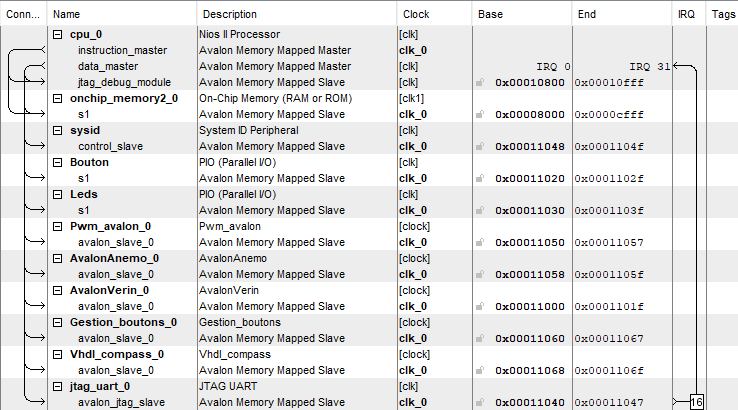
\includegraphics[width=\textwidth]{images/SOPC.png}
      \caption{Les différents composants du SOPC}
    \end{center}
  \end{figure}

  \newpage 

  Une fois les différents composants ajoutés avec leurs différents fichiers VHDL, une boite globale du projet est créée par "SOPC Builder".

  \begin{figure}[h]
    \begin{center}
      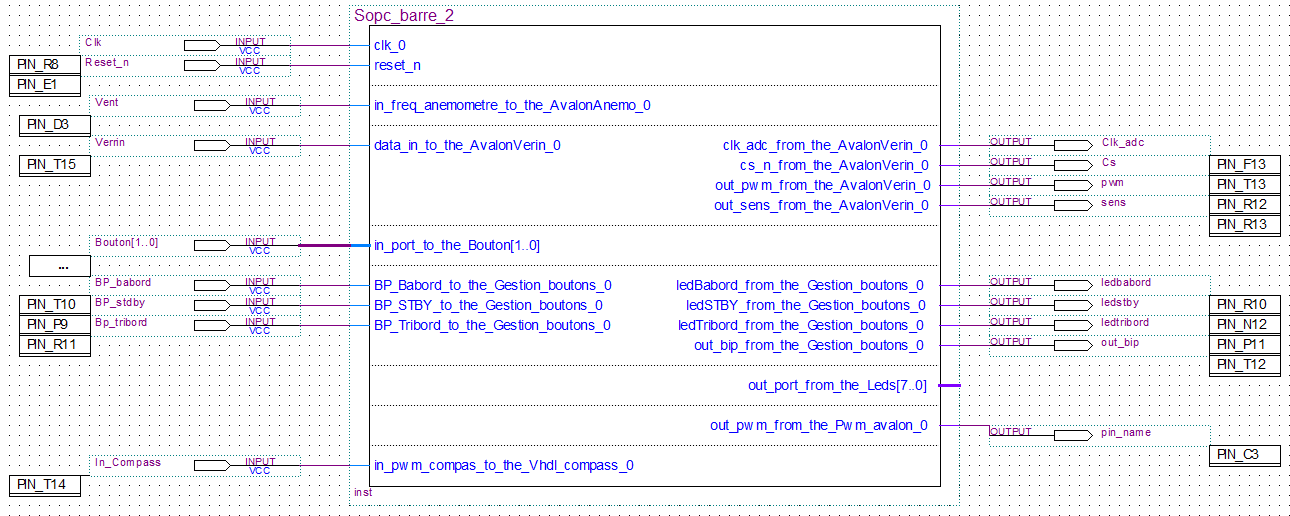
\includegraphics[width=\textwidth]{images/sopc_bloc.png}
      \caption{SOPC et ses différents ports GPIO}
    \end{center}
  \end{figure}


\section{Développement Code Embarqué}
Dans cette section nous présenterons l'utilisation de NIOS II qui est l'outil de développement de Altera permettant la programmation, compilation et le debug du logiciel que nous implémenterons sur le micro-contrôleur de notre FPGA réalisé précédemment (sous environnement Eclipse).\newline


\section{Validation des Fonctions}
Pour effectuer la validation de notre système nous avons téléversé notre projet sur le FPGA, la partie Hardware grâce au SOPC et la partie logicielle à l'aide de l'environnement Eclipse qui nous a permit de lancer/tester et débugger notre projet directement sur la maquette d'évaluation.

\begin{figure}[h]
    \begin{center}
      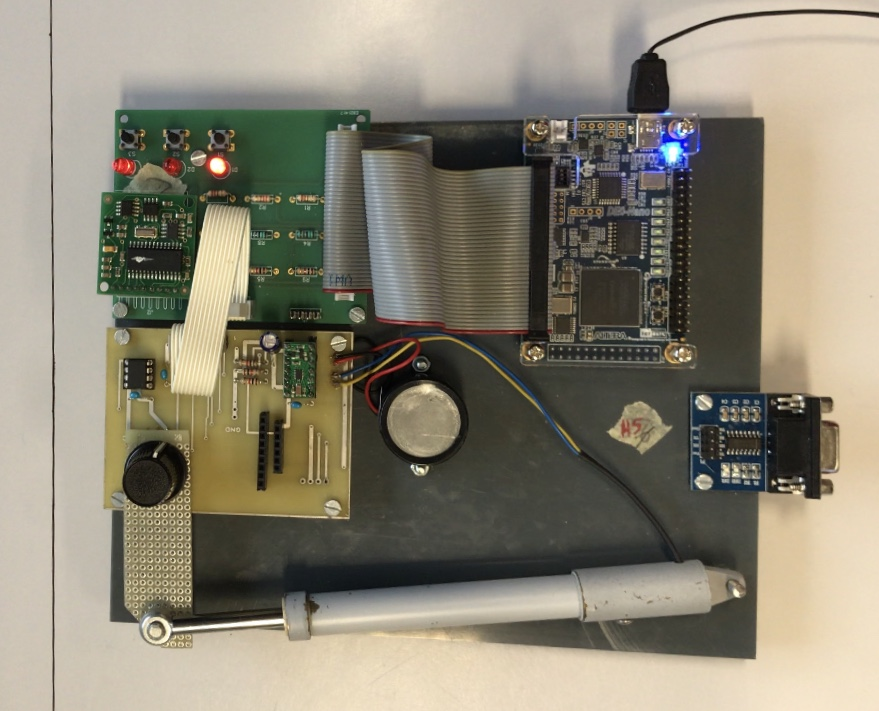
\includegraphics[width=0.7\textwidth]{images/maquette.jpg}
      \caption{Maquette validation projet}
    \end{center}
  \end{figure}

  Nous avons réalisé trois tests pour tester le bon fonctionnement du projet. Pour le premier test nous avons utilisé un GBF qui nous a permit d'injecter directement sur le GPIO, du FPGA attribué, une fréquence qu'on peut modifier pour venir simuler la sortie de l'anémomètre. Après observation la fréquence est bien actualisée toutes les secondes comme demandé dans le cahier des charges. Pour le second test nous venons tester la fonction gestion vérin avec la fonction interface Homme système les boutons nous on permit de tester le bon fonctionnement qui contrôle le signal PWM du vérin. Pour la dernière fonction qui est l'asservissement du système complet nous observons un maintient du cap définit dans le logicielle téléversé sur la maquette de développement et que celle-ci respecte bien le cap fixé avant chaque passage en mode automatique.\newline

  Nous avons aussi testé grâce à l'outil de simulation de Quartus certains composants comme le composant "Div" (Clock\_1Hz), le composant "Detect\_FM" (Détection fronts montants) et la gestion "PWM" important pour la gestion du vérin. Pour cela il faut créer un fichier "Vector Waveform File" et insérer les noeuds que nous souhaitons tester dans l'intervalle de temps, qui doit être adapté pour chaque simulations.
  \newpage
  \subsection{Validation Horloge 1 Hz - Anémomètre}

Une simulation de la fonction "Div" (génération signal 1 Hz) a été réalisée avant implantation, une mesure toute les secondes est nécessaire pour le bon fonctionnement de l'anémomètre c'était donc pour nous une des parties importantes à tester avant de poursuivre le reste du projet.

\begin{figure}[h]
  \begin{center}
    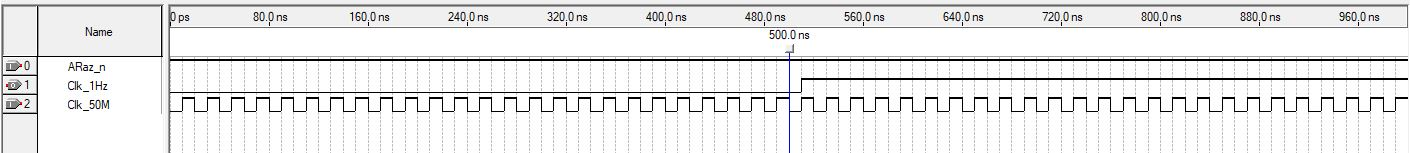
\includegraphics[width=\textwidth]{images/Clk_1Hz.jpg}
    \caption{Simulation du circuit de gestion d'horloge 1 Hz}
  \end{center}
\end{figure}

\subsection{Validation Détecteur Fronts montants - Anémomètre}

Une simulation de la fonction "Detect\_FM" a été réalisée avant implantation, dans cette seconde fonction importante on demande au système de détecter les fronts montants générés par l'anémomètre qui va permettre au système d'informer la vitesse du vent toutes les secondes.

\begin{figure}[h]
  \begin{center}
    \includegraphics[width=\textwidth]{images/Détecteur_Fronts_montants.jpg}
    \caption{Simulation du circuit de détection des fronts montants}
  \end{center}
\end{figure}

\subsection{Validation PWM - Gestion vérin}

Une simulation de la fonction "PWM" a été réalisée avant implantation, dans cette fonction importante de la partie "Gestion vérin" on demande au système de générer un signal PWM qui va être interprété et traité par un composant électronique qui va à son tour piloter le vérin dans un sens ou dans l'autre. Dans cette simulation on observe le bon fonction de celui-ci en faisant varier les valeurs de "Fréquence" et de "Duty".

\begin{figure}[h]
  \begin{center}
    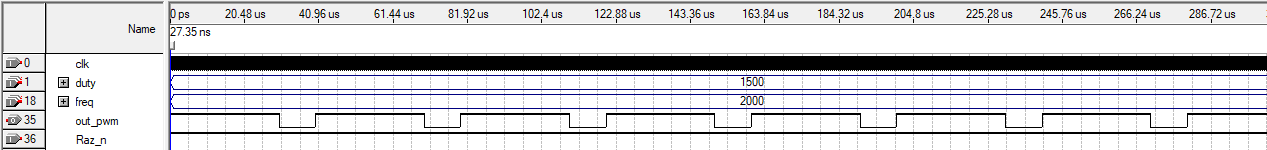
\includegraphics[width=\textwidth]{images/pwm.png}
    \caption{Simulation du circuit de gestion du signal PWM - F = 2000, D = 1500}
  \end{center}
\end{figure}

\section{Conclusion}

\textit{Pour conclure, ce projet fut très enrichissant pour chacun de nous. Il nous as permis de concevoir, valider par la simulation et l’implémentation à partir d’outils appropriés, tout ou une partie des fonctions identifiées lors de la phase d'analyse. Nous avons pu realiser la synthèse et la réalisation de fonctions logiques en langage VHDL, la vérification du fonctionnement en simulation et sur maquette (carte DE2 d’Altera), l’interfacage des composants developpées avec le bus du processeur (bus Avalon et processeur NIOS 32 bits) et pour finir le test et la validation du système complet}\newline
\\

\textit{Ce projet nous as permis d'acquérir des compétences techniques, de mettre en oeuvres les différentes compétences acquises lors de nos cours magistraux et de nous confronter aux difficultés techniques entraînées par la réalisation d'un projet. De pouvoir concevoir, tester et observer un produit développé et réalisé de ses propres mains est quelque chose d'important et qui accorde une grande fierté et satisfaction.}


\clearpage

\end{document}